% SC1007 — Chapter 7: Graphs — Representations, BFS/DFS, MST & Dijkstra Preview
% No \documentclass — included by modules/SC1007/main.tex (book class).
\chapter{Graphs: Representations, Traversals \& Preview}
\label{ch:graphs}

\begin{quote}
\emph{``A graph is just vertices and edges.''} --- Yet it models networks, dependencies, maps, and the web itself.
\end{quote}

\noindent\textbf{Prerequisites:} Ch.~2 (queues/stacks), Ch.~3 (BFS/DFS intuition), Ch.~5 (priority queue for Dijkstra/MST preview).

\section*{Learning Outcomes}
After this chapter you will be able to:
\begin{enumerate}[label=(L\arabic*)]
    \item represent graphs via adjacency matrix vs.\ adjacency list and compare costs;
    \item execute BFS and DFS, classify edges, and analyse $O(n+m)$ time;
    \item implement Union-Find with path compression and union by rank for near-constant amortised set merges;
    \item preview MST (Kruskal/Prim) and Dijkstra's shortest paths at a high level;
    \item model a problem as a graph and choose the right representation.
\end{enumerate}

% ============================================================
\section{Graph Basics \& Representations}
\label{sec:graph-representations}
A graph $G=(V,E)$ has $|V|=n$ vertices and $|E|=m$ edges. Directed vs.\ undirected; weighted vs.\ unweighted. Degree $\deg(v)$ counts incident edges.

Two canonical representations:

\begin{table}[h]
\centering
\small
\begin{tabular}{lcc}
\toprule
Operation & Adj.\ matrix $n\times n$ & Adj.\ list \\
\midrule
Space & $\Theta(n^{2})$ & $\Theta(n+m)$ \\
Edge $(u,v)$ exists? & $O(1)$ & $O(\deg(u))$ \\
List neighbours of $u$ & $\Theta(n)$ scan & $\Theta(\deg(u))$ \\
Sparse $m\ll n^{2}$ & wasteful & efficient \\
Dense $m\approx n^{2}$ & fine & overhead \\
\bottomrule
\end{tabular}
\caption{Adjacency matrix vs.\ list. Choose list for sparse graphs (most real networks).}
\label{tab:graph-repr}
\end{table}

\begin{figure}[h]
\centering
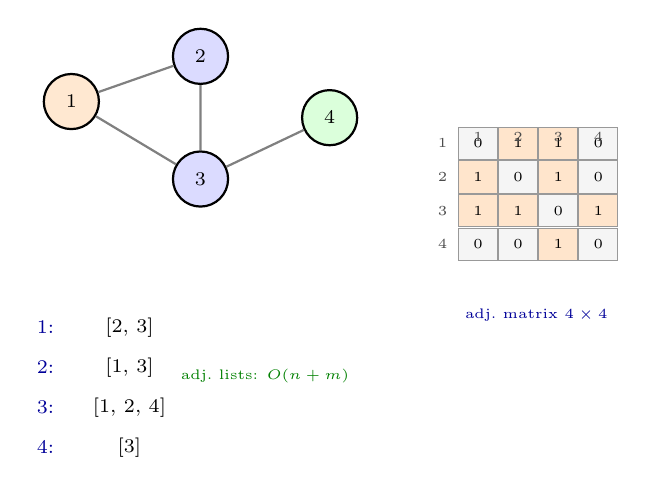
\begin{tikzpicture}[scale=0.82, every node/.style={font=\scriptsize},
  vnode/.style={circle, draw, thick, fill=blue!14, minimum size=0.70cm},
  edge/.style={thick, black!50}]
  % Graph: 4 vertices, edges 1-2, 1-3, 2-3, 3-4 (undirected)
  \node[vnode, fill=orange!18] (1) at (0,1.5) {1};
  \node[vnode] (2) at (2,2.2) {2};
  \node[vnode] (3) at (2,0.3) {3};
  \node[vnode, fill=green!14] (4) at (4,1.25) {4};
  \draw[edge] (1)--(2); \draw[edge] (1)--(3); \draw[edge] (2)--(3); \draw[edge] (3)--(4);
  % Adj matrix (explicit cells)
  \begin{scope}[xshift=6cm, yshift=0.6cm]
    % row 0: 1 connected to 2,3
    \draw[fill=gray!8, draw=black!40] (0,0) rectangle ++(0.60,0.50); \node at (0.30,0.25) {\tiny 0};
    \draw[fill=orange!20, draw=black!40] (0.62,0) rectangle ++(0.60,0.50); \node at (0.92,0.25) {\tiny 1};
    \draw[fill=orange!20, draw=black!40] (1.24,0) rectangle ++(0.60,0.50); \node at (1.54,0.25) {\tiny 1};
    \draw[fill=gray!8, draw=black!40] (1.86,0) rectangle ++(0.60,0.50); \node at (2.16,0.25) {\tiny 0};
    % row 1: 2 connected to 1,3
    \draw[fill=orange!20, draw=black!40] (0,-0.52) rectangle ++(0.60,0.50); \node at (0.30,-0.27) {\tiny 1};
    \draw[fill=gray!8, draw=black!40] (0.62,-0.52) rectangle ++(0.60,0.50); \node at (0.92,-0.27) {\tiny 0};
    \draw[fill=orange!20, draw=black!40] (1.24,-0.52) rectangle ++(0.60,0.50); \node at (1.54,-0.27) {\tiny 1};
    \draw[fill=gray!8, draw=black!40] (1.86,-0.52) rectangle ++(0.60,0.50); \node at (2.16,-0.27) {\tiny 0};
    % row 2: 3 connected to 1,2,4
    \draw[fill=orange!20, draw=black!40] (0,-1.04) rectangle ++(0.60,0.50); \node at (0.30,-0.79) {\tiny 1};
    \draw[fill=orange!20, draw=black!40] (0.62,-1.04) rectangle ++(0.60,0.50); \node at (0.92,-0.79) {\tiny 1};
    \draw[fill=gray!8, draw=black!40] (1.24,-1.04) rectangle ++(0.60,0.50); \node at (1.54,-0.79) {\tiny 0};
    \draw[fill=orange!20, draw=black!40] (1.86,-1.04) rectangle ++(0.60,0.50); \node at (2.16,-0.79) {\tiny 1};
    % row 3: 4 connected to 3
    \draw[fill=gray!8, draw=black!40] (0,-1.56) rectangle ++(0.60,0.50); \node at (0.30,-1.31) {\tiny 0};
    \draw[fill=gray!8, draw=black!40] (0.62,-1.56) rectangle ++(0.60,0.50); \node at (0.92,-1.31) {\tiny 0};
    \draw[fill=orange!20, draw=black!40] (1.24,-1.56) rectangle ++(0.60,0.50); \node at (1.54,-1.31) {\tiny 1};
    \draw[fill=gray!8, draw=black!40] (1.86,-1.56) rectangle ++(0.60,0.50); \node at (2.16,-1.31) {\tiny 0};
    \node[font=\tiny, gray!60!black] at (-0.25, 0.25) {1};
    \node[font=\tiny, gray!60!black] at (-0.25,-0.27) {2};
    \node[font=\tiny, gray!60!black] at (-0.25,-0.79) {3};
    \node[font=\tiny, gray!60!black] at (-0.25,-1.31) {4};
    \node[font=\tiny, gray!60!black] at (0.30, 0.35) {1};
    \node[font=\tiny, gray!60!black] at (0.92, 0.35) {2};
    \node[font=\tiny, gray!60!black] at (1.54, 0.35) {3};
    \node[font=\tiny, gray!60!black] at (2.16, 0.35) {4};
    \node[font=\tiny, blue!60!black] at (1.2,-2.4) {adj.\ matrix $4\times4$};
  \end{scope}
  % Adj list
  \begin{scope}[yshift=-2.0cm, xshift=0.2cm]
    \node[font=\scriptsize, blue!60!black] at (-0.6,0) {1:};
    \node[font=\scriptsize] at (0.7,0) {[2, 3]};
    \node[font=\scriptsize, blue!60!black] at (-0.6,-0.62) {2:};
    \node[font=\scriptsize] at (0.7,-0.62) {[1, 3]};
    \node[font=\scriptsize, blue!60!black] at (-0.6,-1.24) {3:};
    \node[font=\scriptsize] at (0.7,-1.24) {[1, 2, 4]};
    \node[font=\scriptsize, blue!60!black] at (-0.6,-1.86) {4:};
    \node[font=\scriptsize] at (0.7,-1.86) {[3]};
    \node[font=\tiny, green!50!black] at (2.8,-0.75) {adj.\ lists: $O(n+m)$};
  \end{scope}
\end{tikzpicture}
\caption{Undirected graph with 4 vertices, 4 edges: adjacency matrix (symmetric, orange $=1$) vs.\ adjacency lists.}
\label{fig:graph-representations}
\end{figure}

Implementation: matrix as \texttt{vector<vector<int>>} or bitset;\ list as \texttt{vector<vector<int>>} (weighted variant uses\ \texttt{pair<int,int>} for $(v,w)$).

\begin{lstlisting}[language=Python]
# Adjacency list -- Python
n = 4
adj = [[] for _ in range(n)]
def add_edge(u, v, w=1):  # 0-indexed, undirected
    adj[u].append((v, w))
    adj[v].append((u, w))
add_edge(0,1); add_edge(0,2); add_edge(1,2); add_edge(2,3)
# adj[2] == [(0,1),(1,1),(3,1)]
\end{lstlisting}

% ============================================================
\section{BFS \& DFS}
\label{sec:bfs-dfs}
Both traverse in $O(n+m)$ with adjacency lists ($O(n^{2})$ with matrix).

\textbf{BFS} uses a queue: explores in increasing distance from source. Yields shortest paths (fewest edges) in unweighted graphs. Records \texttt{dist} and \texttt{parent}.

\textbf{DFS} uses a stack (recursion): goes deep before backtracking. Classifies edges as tree/back/forward/cross (directed case). Useful for topological sort and cycle detection.

\begin{figure}[h]
\centering
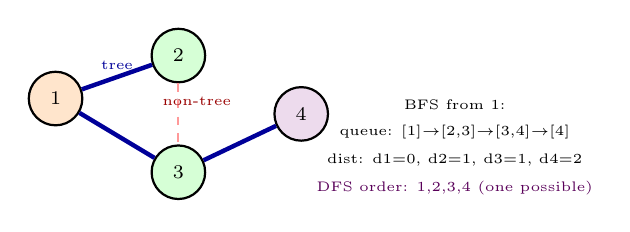
\begin{tikzpicture}[scale=0.78, every node/.style={font=\scriptsize},
  vnode/.style={circle, draw, thick, fill=blue!14, minimum size=0.68cm},
  edge/.style={thick, black!35}]
  % Same graph, BFS tree highlighted
  \node[vnode, fill=orange!20] (1) at (0,1.5) {1};
  \node[vnode, fill=green!16] (2) at (2,2.2) {2};
  \node[vnode, fill=green!16] (3) at (2,0.3) {3};
  \node[vnode, fill=violet!14] (4) at (4,1.25) {4};
  \draw[edge, ultra thick, blue!60!black] (1)--(2);
  \draw[edge, ultra thick, blue!60!black] (1)--(3);
  \draw[edge, thick, red!40, dashed] (2)--(3);
  \draw[edge, ultra thick, blue!60!black] (3)--(4);
  \node[font=\tiny, blue!60!black] at (1,2.05) {tree};
  \node[font=\tiny, red!60!black] at (2.3,1.45) {non-tree};
  \begin{scope}[xshift=6.5cm, yshift=0.8cm]
    \node[font=\tiny, align=left] at (0,0.6) {BFS from 1:};
    \node[font=\tiny, align=left] at (0,0.15) {queue: [1]$\to$[2,3]$\to$[3,4]$\to$[4]};
    \node[font=\tiny, align=left] at (0,-0.3) {dist: d1=0, d2=1, d3=1, d4=2};
    \node[font=\tiny, align=left, violet!70!black] at (0,-0.75) {DFS order: 1,2,3,4 (one possible)};
  \end{scope}
\end{tikzpicture}
\caption{BFS tree from vertex 1 (blue thick = tree edges). Dashed edge (2,3) is non-tree; BFS finds shortest-path distances.}
\label{fig:bfs-tree}
\end{figure}

\begin{lstlisting}[language=Python]
from collections import deque
def bfs(adj, s):
    n = len(adj)
    dist = [-1]*n; parent = [-1]*n
    dist[s]=0; q=deque([s])
    order=[]
    while q:
        u=q.popleft(); order.append(u)
        for v,_ in adj[u]:
            if dist[v]==-1:
                dist[v]=dist[u]+1; parent[v]=u; q.append(v)
    return order, dist, parent

def dfs(adj, s, visited=None, order=None):
    if visited is None: visited=set(); order=[]
    visited.add(s); order.append(s)
    for v,_ in adj[s]:
        if v not in visited: dfs(adj, v, visited, order)
    return order
\end{lstlisting}

\begin{figure}[h]
\centering
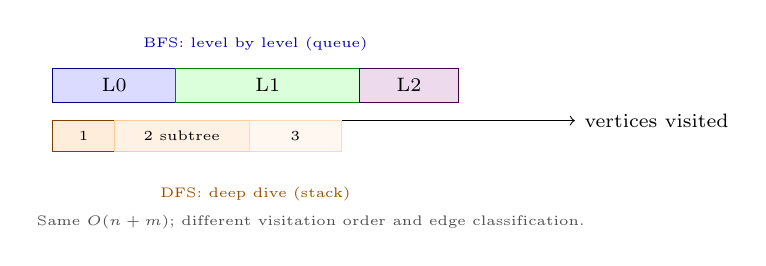
\begin{tikzpicture}[scale=0.78, every node/.style={font=\scriptsize}]
  % Time bars for BFS vs DFS
  \draw[->] (0,0) -- (8.5,0) node[right] {vertices visited};
  \draw[fill=blue!14, draw=blue!50!black] (0,0.3) rectangle ++(2.0,0.55) node[midway] {L0};
  \draw[fill=green!14, draw=green!50!black] (2.0,0.3) rectangle ++(3.0,0.55) node[midway] {L1};
  \draw[fill=violet!14, draw=violet!50!black] (5.0,0.3) rectangle ++(1.6,0.55) node[midway] {L2};
  \node[font=\tiny, blue!60!black] at (3.3,1.25) {BFS: level by level (queue)};
  \draw[fill=orange!14, draw=orange!50!black] (0,-0.5) rectangle ++(1.0,0.50) node[midway, font=\tiny] {1};
  \draw[fill=orange!10, draw=orange!40] (1.0,-0.5) rectangle ++(2.2,0.50) node[midway, font=\tiny] {2 subtree};
  \draw[fill=orange!6, draw=orange!30] (3.2,-0.5) rectangle ++(1.5,0.50) node[midway, font=\tiny] {3};
  \node[font=\tiny, orange!60!black] at (3.3,-1.2) {DFS: deep dive (stack)};
  \node[font=\tiny, gray!60!black] at (4.2,-1.65) {Same $O(n+m)$; different visitation order and edge classification.};
\end{tikzpicture}
\caption{BFS vs.\ DFS visitation pattern on the same graph. BFS is level-order; DFS plunges deep.}
\label{fig:bfs-vs-dfs}
\end{figure}

% ============================================================
\section{Union-Find: Merging Sets Almost for Free}
\label{sec:union-find}
\emph{Intuition:} Kruskal grows connected components by merging sets. Each set elects a \emph{representative} (leader): \textsc{Find}$(x)$ asks ``who leads $x$'s set?'' and \textsc{Union}$(x,y)$ merges two sets. Membership trees make both fast: \textsc{Find} climbs to the root, \textsc{Union} attaches the shorter tree under the taller (\emph{union by rank}) while shortcutting every visited node to the root (\emph{path compression}).
\begin{lstlisting}[language=Python]
parent = list(range(n)); rank = [0]*n
def find(x):
    while parent[x] != x: parent[x] = parent[parent[x]]; x = parent[x]
    return x  # halving: each step skips a level
def union(x, y):
    rx, ry = find(x), find(y)
    if rx == ry: return False  # already connected: edge would close a cycle
    if rank[rx] < rank[ry]: parent[rx] = ry
    else: parent[ry] = rx; rank[rx] += (rank[rx] == rank[ry])
    return True
\end{lstlisting}
\begin{example}[Worked] $n=5$: \textsc{Union}$(1,2)$ and \textsc{Union}$(3,4)$ build $\{1,2\},\{3,4\}$; \textsc{Union}$(2,3)$ attaches root $3$ under $1$ (equal rank, one grows). A later \textsc{Find}$(4)$ climbs $4\to3\to1$, then compression links $4$ directly to $1$. Any sequence of $m$ operations costs $O(m\,\alpha(n))$ with $\alpha$ the inverse Ackermann function ($\le5$ for every realistic $n$) --- effectively constant, which is why Kruskal's sort dominates its $O(m\log n)$.
\end{example}

% ============================================================
\section{Preview: MST \& Shortest Paths}
\label{sec:mst-dijkstra-preview}
\textbf{Minimum Spanning Tree (MST):} cheapest set of $n-1$ edges connecting all vertices. Kruskal sorts edges and merges components with Union-Find (Sec.~\ref{sec:union-find}); Prim grows via min-heap (Ch.~5): both $O(m\log n)$.

\textbf{Dijkstra:} single-source shortest paths for non-negative weights. Repeatedly extracts min-distance vertex from a heap and relaxes edges: $O((n+m)\log n)$ with binary heap. BFS is the special case $w=1$.

These are developed fully in SC2001; here we note that the right heap + graph representation gives the right bound.

% ============================================================
\section{Chapter Notes}
CLRS Ch.~20--24, Weiss Ch.~9. Adj.\ list is default for sparse graphs; matrix for dense or fast edge queries. BFS/DFS are the workhorses for connectivity, bipartiteness, and topological sort.

% ============================================================
\section{Exercises}
\label{sec:ch07-exercises}
\begin{enumerate}[label=E7.\arabic*, leftmargin=*, itemsep=0.7em]
    \item \textbf{Representations.} For $n=1000$, $m=3000$, compute space for matrix (1 byte/entry) vs.\ list (8 bytes/edge endpoint). At what $m$ does matrix win?
    \item \textbf{BFS distances.} Run BFS from vertex 1 on Fig.~\ref{fig:graph-representations}. Give \texttt{dist}, \texttt{parent}, and BFS tree. Prove BFS indeed gives shortest-path distances in unweighted graphs.
    \item \textbf{DFS classification.} Run DFS from 1 on the same graph (neighbour order increasing). Classify each edge as tree/back/forward/cross (treat undirected edges as two directed arcs).
    \item \textbf{Dijkstra preview.} Add weights $w(1,2)=4,w(1,3)=2,w(2,3)=1,w(3,4)=5$. Run Dijkstra from 1 by hand with a heap; show extract order and final distances. Why does negative weight break it?
    \item \textbf{MST preview.} Give MST of the weighted graph above (list edges and total weight). Run Kruskal and Prim and compare steps.
\end{enumerate}
% End of Chapter 7
